\chapter{Estudo de Caso B --- Ciclismo com Eletroestimulação Funcional}
\label{cap:caso-trike}

Este capítulo apresenta o segundo estudo de caso: o sistema de ciclismo assistido por
eletroestimulação funcional (FES \emph{Cycling}) do Projeto EMA. Diferentemente do sistema
de realidade virtual, trata-se de um sistema \emph{ativo}, com equipe atualmente
trabalhando sobre ele --- o que não o isenta, contudo, das mesmas fragilidades de
Engenharia de Software. O capítulo documenta o que o sistema é
(Seção~\ref{sec:trike-oque}), a sua arquitetura atual (Seção~\ref{sec:trike-asis}), a
tentativa de reprodução (Seção~\ref{sec:trike-reproducao}) e as limitações específicas
identificadas (Seção~\ref{sec:trike-limitacoes}).

\section{Visão Geral do Sistema}
\label{sec:trike-oque}

O sistema controla um triciclo reclinado (\emph{trike}) adaptado, em configuração
\emph{tadpole}, no qual a pedalada é produzida pela estimulação elétrica de músculos
paralisados ou enfraquecidos do ciclista. Um sensor inercial mede o ângulo do pedal
(\emph{crank}) e, a partir dele, uma lógica de controle determina quais grupos musculares
estimular e em que instante, de modo a produzir uma pedalada coordenada e segura
\cite{brindeiro2017,baptista2022}. O sistema é herdeiro de uma linha de pesquisa consolidada
do laboratório, que inclui a participação da equipe na competição internacional CYBATHLON e
o emprego de técnicas avançadas de estimulação centradas no usuário \cite{baptista2022}. A
Figura~\ref{fig:trike-foto} apresenta o sistema e a sua arquitetura de controle, tal como
documentados.

\begin{figure}[H]
	\centering
	\caption{Sistema de ciclismo com FES: (a) montagem física; (b) arquitetura de controle em nós.}
	\label{fig:trike-foto}
	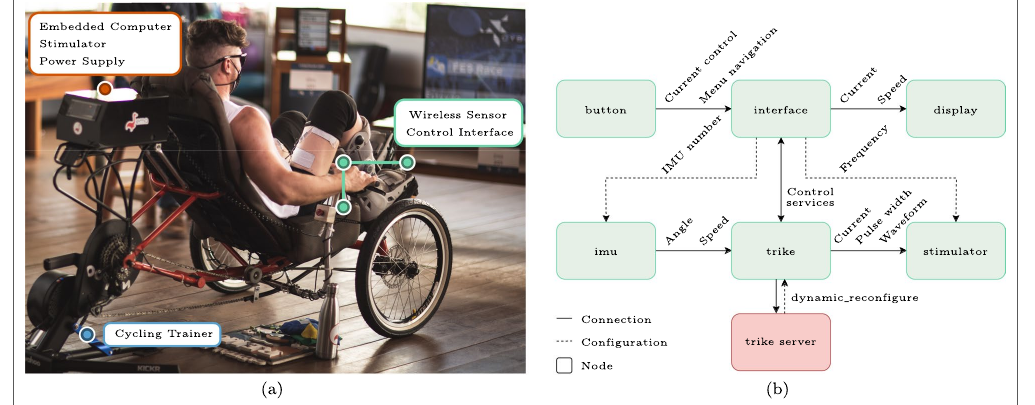
\includegraphics[width=0.98\textwidth]{figuras/trike_sistema_baptista}

	\vspace{4pt}
	{\footnotesize Fonte: \citeonline{baptista2022}.}
\end{figure}

Conforme documentado, o núcleo de processamento é um computador embarcado (Raspberry Pi), ao
qual se conectam um eletroestimulador multicanal, um sensor inercial sem fio que mede o
ângulo do \emph{crank} e uma interface humano-máquina (HMI) composta por botões físicos e um
display LCD. A interação com o operador e o atleta é mediada por essa HMI.

\subsection{Dois Repositórios, Duas Gerações}
\label{sec:trike-repos}

Um aspecto essencial para compreender este estudo de caso --- e um achado de diagnóstico em
si --- é que o sistema existe hoje sob duas gerações tecnológicas, em dois repositórios
distintos:

\begin{itemize}
	\item \texttt{ema\_fes\_cycling} (público) --- a implementação \textbf{original em
	      ROS~1}, à qual corresponde a arquitetura documentada da
	      Figura~\ref{fig:trike-foto}. Este repositório é razoavelmente documentado: possui
	      \texttt{README}, \emph{Wiki} com guias de instalação (para PC e para Raspberry Pi)
	      e de primeiros passos, licença definida e versões marcadas (\emph{releases}).
	      Reflete, porém, uma geração tecnológica anterior.
	\item \texttt{ema\_fes\_ros2} (privado) --- a \textbf{reescrita em ROS~2}, que constitui
	      a linha de desenvolvimento ativa. Ao contrário do original, este repositório
	      praticamente não dispõe de documentação: o \texttt{README} resume-se a poucas
	      linhas de anotações técnicas, sem guia de instalação ou de execução.
\end{itemize}

Esse desdobramento evidencia um fenômeno recorrente: a migração de ROS~1 para ROS~2 produziu
um novo repositório que \emph{perdeu} a documentação que o original possuía, além de
fragmentar a mesma linha de trabalho em dois artefatos com estados de documentação opostos.
A tentativa de reprodução descrita adiante refere-se à geração ativa (ROS~2).

\section{Arquitetura Atual (As-Is)}
\label{sec:trike-asis}

A arquitetura de controle apoia-se no modelo de nós e tópicos do ROS descrito na
Seção~\ref{sec:ros}, ilustrado na Figura~\ref{fig:trike-foto}(b). Na versão documentada, os
nós dividem-se por função: um nó de botões e um nó de \emph{display} compõem a HMI; um nó de
interface interpreta os comandos e gerencia a navegação; um nó de IMU publica o ângulo e a
velocidade do \emph{crank}; e um nó central de controle calcula os instantes de estimulação a
partir do ângulo e da velocidade e envia ao nó do estimulador os parâmetros de corrente,
largura de pulso e forma de onda. Na reescrita ativa em ROS~2, essa lógica de controle está a
cargo dos nós \texttt{control\_node} e \texttt{control\_shift\_node}, ao lado de
\texttt{imu\_node}, \texttt{stim\_node} e \texttt{hmi\_node}, preservando a mesma divisão de
responsabilidades.

A lógica de decisão do controle apoia-se em faixas angulares: para cada grupo muscular,
definem-se um ângulo inicial de estimulação e uma amplitude, de modo que o ângulo final de
parada seja $\texttt{stop\_angles} = \texttt{start\_angles} + \texttt{angle\_range}$;
verifica-se, a cada instante, se a posição do pedal está na zona de estimulação ou na zona de
parada. Por assentar-se no ROS~2, a versão ativa dispõe, em princípio, dos mecanismos de
Qualidade de Serviço e de segurança discutidos na Seção~\ref{sec:ros} --- como a
diferenciação entre telemetria tolerante a perdas e comandos de entrega garantida, e
salvaguardas que coloquem o estimulador em modo seguro caso o nó de controle deixe de emitir
comandos válidos. Cabe ressalvar, todavia, que o uso pleno dessas salvaguardas figura, no
material analisado, mais como \emph{plano} do que como implementação confirmada; a sua
efetivação é uma das recomendações do Capítulo~\ref{cap:proposta}.

\subsection{Lacuna entre o Registrado e o Montado}

Um achado central deste estudo de caso é a divergência entre a arquitetura documentada e a
efetivamente montada. A interface humano-máquina, por exemplo, depende de um
microcontrolador (ESP32 ou Arduino) que se comunica com o computador embarcado; o
\emph{display} constitui, na prática, um componente que troca dados com esse
microcontrolador. Contudo, tais elementos não figuram de forma completa nos diagramas de
referência preexistentes, o que caracteriza um diagrama \emph{incompleto} em relação ao
hardware real. Essa é uma manifestação concreta da lacuna entre o que está registrado e o
que está montado, e um dos pontos que a diagramação padronizada proposta neste trabalho
busca corrigir.

\section{Tentativa de Reprodução}
\label{sec:trike-reproducao}

A tentativa de executar a geração ativa (ROS~2, repositório \texttt{ema\_fes\_ros2}) tal
como se encontra revelou uma sucessão de obstáculos, aqui registrados como dados de
diagnóstico:

\begin{itemize}
	\item \textbf{Ausência de documentação no repositório ativo:} o repositório da reescrita
	      em ROS~2 não traz documentação que oriente a execução, restando a descoberta manual
	      dos modos de funcionamento por tentativa e erro.
	\item \textbf{Falha na execução conteinerizada:} a tentativa natural de subir o sistema
	      via \texttt{docker compose} esbarra na referência a uma imagem específica que não
	      está publicada em lugar algum, obrigando a improvisar com uma versão aproximada.
	\item \textbf{Restrições rígidas de ambiente:} a versão do ROS~2 empregada exige um
	      sistema operacional específico (Ubuntu 22.04, com Python 3.10 e bibliotecas
	      compatíveis), o que torna o ambiente pouco portável.
	\item \textbf{Hierarquia de inicialização rígida:} existe um arquivo ``inicializador''
	      concebido para ``facilitar'' a partida do sistema, mas que, na prática, dificulta
	      a depuração: os nós ficam à espera de parâmetros de configuração oriundos dessa
	      inicialização e não podem ser executados isoladamente, forçando uma operação de
	      ``tudo ou nada''.
	\item \textbf{Código-fonte ausente:} falta um dos códigos mais importantes ---
	      o da interface humano-máquina (HMI), que depende apenas de um ESP32 ou Arduino ---,
	      cuja ausência impede inclusive a depuração do que ocorre durante o treino.
	\item \textbf{Documentação de infraestrutura incompleta:} a documentação existente
	      menciona um servidor do EMA e recursos de acesso remoto e telemetria que são
	      praticamente impossíveis de reimplementar, por não haver descrição de como
	      configurá-los.
	\item \textbf{Tentativa em plataforma alternativa:} uma tentativa de instalação manual
	      em uma Raspberry Pi~4B (sem Docker, para não onerar o hardware) esbarrou novamente
	      na hierarquia de inicialização, que impediu a execução individual dos nós para fins
	      de depuração.
\end{itemize}

O conjunto desses obstáculos sustenta a resposta à pergunta-guia do trabalho: na geração
ativa e nas condições atuais, o sistema \emph{não} pode ser reproduzido por um novo
integrante sem esforço considerável de engenharia reversa e sem acesso a conhecimento tácito
não documentado --- e isso apesar de a geração anterior (ROS~1) dispor de guias de
instalação.

\section{Limitações Específicas Identificadas}
\label{sec:trike-limitacoes}

\begin{itemize}
	\item \textbf{Documentação perdida na migração:} a reescrita ativa em ROS~2 não herdou a
	      documentação (\texttt{README}, \emph{Wiki}, guias) que o repositório original em
	      ROS~1 possui.
	\item \textbf{Código-fonte incompleto:} ausência do código da HMI (ESP32/Arduino),
	      essencial para a operação e a depuração do treino.
	\item \textbf{Reprodutibilidade comprometida:} dependência de imagem de contêiner
	      inexistente e de ambiente rígido, sem passo a passo de instalação no repositório
	      ativo.
	\item \textbf{Acoplamento na inicialização:} hierarquia de \emph{launch} que impede a
	      execução isolada de nós, dificultando testes e depuração.
	\item \textbf{Documentação de hardware ausente:} inexistência de um diagrama de hardware
	      que permita replicar o sistema para testes ou manutenções.
	\item \textbf{Infraestrutura não documentada:} servidor e recursos de telemetria/acesso
	      remoto sem documentação de configuração.
	\item \textbf{Incoerência entre diagramas e hardware:} componentes reais (como o
	      \emph{display} conectado ao microcontrolador) ausentes dos diagramas de referência.
\end{itemize}
